\newcommand{\bigdatachapter}{Kapitel 9. }
\chapter{Big Data}
\label{chapter:big-data}
\lhead{\bigdatachapter \emph{Big Data}}

\section{Allgemein}
Wir haben in unserem Projekt ein großes Augenmerk auf das Sammeln von Daten gelegt. Big Data ist ein Thema, auf welches man in Zeiten wie diesen, in immer mehr Bereichen des Lebens stößt. Sei es die Kontaknachverfolgung, die Digitalisierung sämtlicher gesundheitlicher und behördlicher Dokumente, oder das Sammeln von Kundendaten.

Wir und unser Projekt zählt sich eher zum Letzteren und da wir nun schon auf die Quelle der Daten, Pepper und seine Kommunikation mit den Studenten und Interessierten, sowie auf die Verarbeitung und Speicherung mit Hilfe unserer Webanwendung eingegangen sind, wollen wir nun auch noch einmal aufzeigen, was man mit diesen Informationen anfangen kann. Einen kleinen Ausschnitt haben wir schon in den Abbildungen \ref{fig:admindashboard1}, \ref{fig:admindashboard2} und \ref{fig:webappdetail} gesehen. Doch dort ist nicht mehr, als die bloße Einsicht möglich.\\

\section{Datenanalyse mit Python und Jupyter Notebook}
Hier kam es uns zu Gute, dass wir uns mit Jupyter Notebooks sehr gut auskennen. Wir haben eine Client Klasse in Python geschrieben, welche es uns ermöglicht, durch bloße Eingabe des API Keys, auf Daten in unserer Webanwendung zuzugreifen. Hierfür wird der Endpunkt \verb|/docker-hbv-kms-http/api/v1/sql| angesprochen, an welchen wir unsere SQL Abfragen schicken können und die Ergebnisse als Antwort von unserer Webanwendung zurück bekommen.

Die Client Klasse sorgt automatisch dafür, dass die Anfragen entsrechend formatiert und abgeschickt werden, sowie Fehler ohne Probleme behandelt und mitgeteilt werden. Somit bekommt der Nutzer in seinem Jupyter Notebook mitgeteilt, sofern er einen Fehler in seiner SQL Syntax hat, da wir auch diese Informationen von unserem Server an den Benutzer übermitteln. Nachfolgend ist ein solches Beispiel vorgeführt:
\newpage

\begin{lstlisting}[language=Python]
    [ IN ]  client = Client(API_KEY, sandbox=False)
    [ OUT ] { 'message': 'Connected!' }
    [ IN ]  client.sql_query('select * from users')
    [ OUT ] Exception: 400-Invalid SQL command!
\end{lstlisting}

Wer sich an Abschnitt \ref{sec:api-sql-query} erinnert wird bemerken, dass die Tabelle \verb|users| nicht über diesen Endpunkt ansprechbar ist.

Der Parameter \verb|sandbox|, welcher im Konstruktor der Client Klasse verarbeitet wird, gibt an, ob sich mit der lokalen Instanz der Webanwendung, oder mit der in der Produktivumgebung verbinden werden soll.

Hat man nun die Client Klasse instantiiert, ist es mit ihr möglich eine Vielzahl von SQL Abfragen durchzuführen, um an verschiedene von Pepper gespeicherte Konversationsdaten zu gelangen.

Mit Hilfe der Bibliotheken Pandas, Matplotlib und weiteren Frameworks, haben wir innerhalb dieses Notebooks verschiedene Visualisierungen angefertigt. Hierbei ist zu beachten, dass all diese Daten mit Hilfe des Skriptes aus Abschnitt \ref{sec:dummy-data} generiert worden sind.\\

\begin{figure}[H]
    \centering
    \begin{minipage}[b]{0.49\textwidth}
        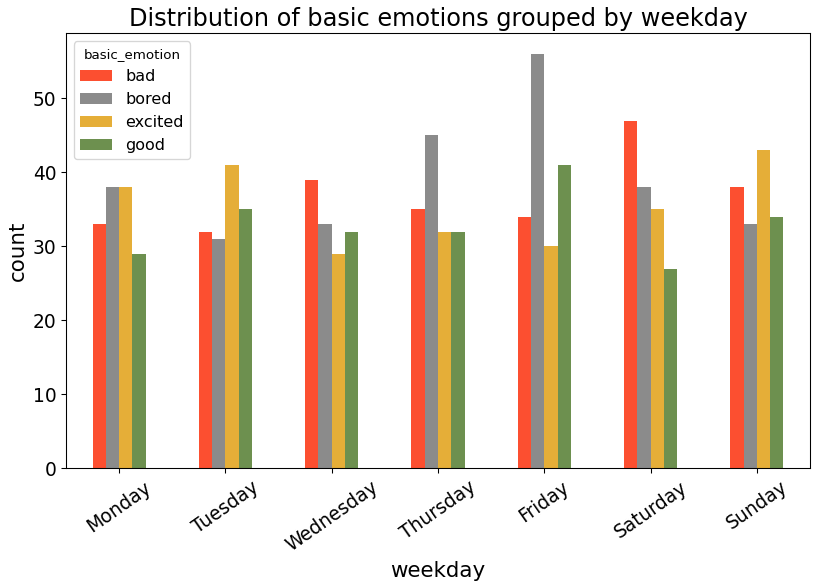
\includegraphics[width=\textwidth]{Figures/analysis/emotionwd.png}
        \caption{Diagramm: Emotion je Wochentag}
        \label{fig:emotionwd}
    \end{minipage}
    \hfill
    \begin{minipage}[b]{0.49\textwidth}
        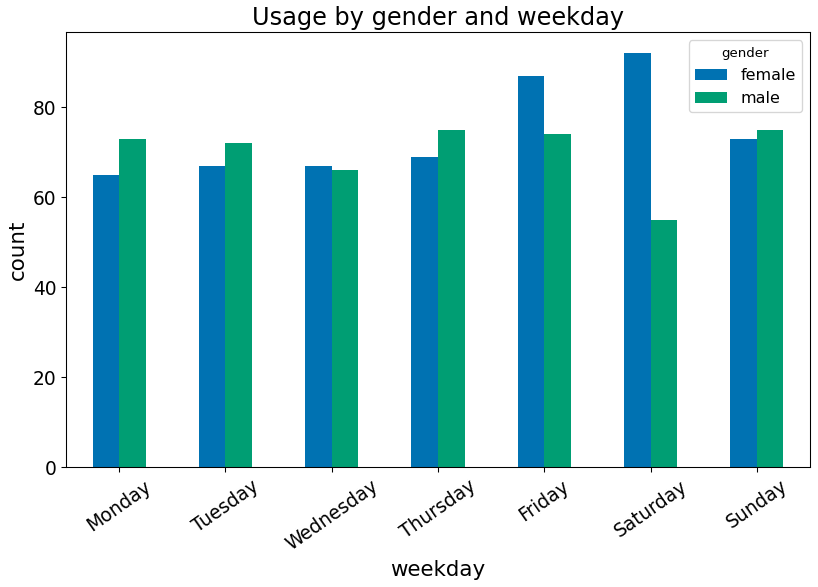
\includegraphics[width=\textwidth]{Figures/analysis/genderwd.png}
        \caption{Diagramm: Geschlecht je Wochentag}
        \label{fig:genderwd}
    \end{minipage}
\end{figure}

\begin{figure}[H]
    \centering
    \begin{minipage}[b]{0.49\textwidth}
        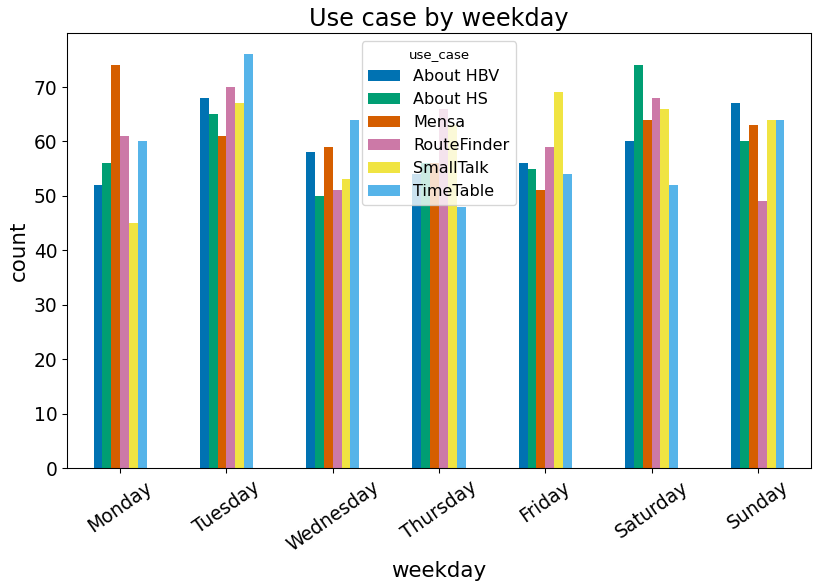
\includegraphics[width=\textwidth]{Figures/analysis/usecasewd.png}
        \caption{Diagramm: UseCase je Wochentag}
        \label{fig:usecasewd}
    \end{minipage}
    \hfill
    \begin{minipage}[b]{0.49\textwidth}
        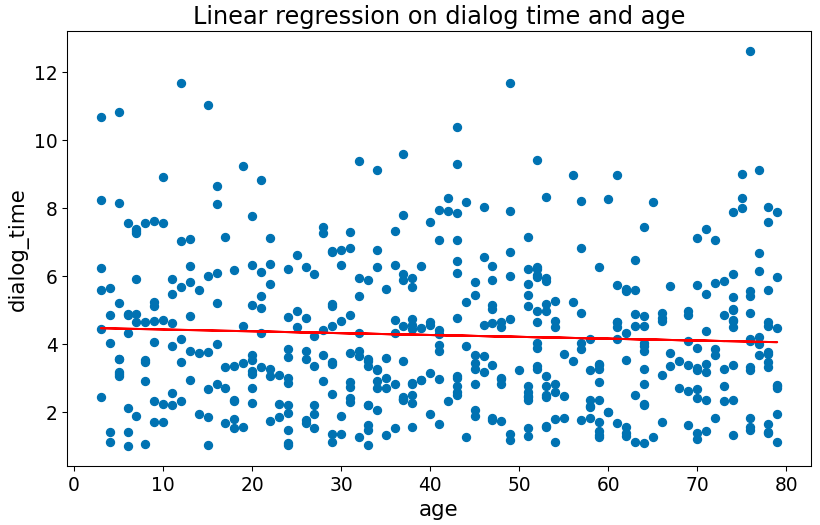
\includegraphics[width=\textwidth]{Figures/analysis/linreg.png}
        \caption{Diagramm: Lineare Regression zwischen Dialog Zeit und Alter}
        \label{fig:linreg}
    \end{minipage}
\end{figure}

Die Abbildungen \ref{fig:emotionwd}ff. geben einen kleinen Vorgeschmack auf die Möglichkeiten der Analyse der von Pepper sammelbaren Daten. In dem Notebook sind weitere Diagramme zu finden, auch ein simples RNN wurde konstruiert, mit welchem wir das Alter anhand der zur Verfügung stehenden Parameter bestimmen wollten. Jedoch es nicht verwunderlich, dass wir bei einer Genauigkeit von 50\% liegen, da diese Daten von uns generiert worden sind.

Diese Schnittstelle zu unserem Webserver ermölgicht es dem Anwender, einen genaueren Einblick in die Daten zu bekommen. Zusätzlich zu diesem Notebook, haben wir ein Skript erstellt, welches die Daten aus der Datenbank abruft und die Visualisierungen als PDF Datei speichert. Dies ist in Verbindung mit einem Cronjob, einem wiederkehrenden Prozess, sehr nützlich. So können wir, aber auch andere, die diese Art der Anwendung nutzen wollen, sich in regelmäßigen Abständen, Berichte generieren lassen, welche einen tieferen Einblick in die Daten bieten.

Durch die Anbindung von Pepper an unsere Webanwendung ist es möglich, sämtliche Informationen, während einer Konversation zu speichern und nachzuvollziehen. Hiermit können Unternehmen herausfinden, was ihre Kunden bewegt und in welchen Bereichen man noch an seinem Geschäftsmodell arbeiten muss. Es wäre denkbar, mehrere Pepper, welche den selben Datensammlungsablauf haben, an verschiedene Unternehmen zu vermieten, womit man als Vermittler ein großes Kontingent an Informationen zu verschiedenen Branchen sammeln und auswerten kann.\\

